\section{Project Management}\label{project-sec}

This project is, among other things, an experiment on how to organise large scale collaborations for mathematical work. In this section, we describe several aspects of the organisation of the collaborative effort.

\subsection{Problems of scale in mathematical collaboration}
In order to understand the scaling issues that can arise in large scale collaborations, it helps to revisit the mechanics of traditional mathematical collaborations and their limitations. While every collaboration is unique, there are some general patterns. A small number of contributors, usually under ten, who may know each other, join forces to tackle some class of problems. Typically the collaborators are almost all academics who share substantial amounts of common knowledge. They discuss the problem at hand together, typically with some shared written medium such as a whiteboard. After several rounds of discussion and refinement, different members of the collaboration come up with different pieces of a solution. These pieces are then put together via discussion and merging of write-ups over several iterations. Once the collaborators are reasonably confident about the correctness of their work, including theorem statements and proofs, they submit the paper for peer review. Thus the correctness of mathematical research relies on this basic cycle of discuss, solve, write, cross-check, and revise, followed by peer review. Ultimately the authors take responsibility for the contents of their research article. This joint responsibility for authorship is formally enshrined by mathematical societies. For instance, see point 4 of the EMS code of practice for joint responsibility \cite{EMS_code_of_practice}.

However this project involved over fifty contributors spread across the world with diverse academic and professional backgrounds. They collaborated across several timezones and countries over the internet. The aforementioned process does not scale. Collaborators do not usually know each other nearly as well as they would in a traditional project. Thus such a collaboration does not have the same level of mutual trust. Further, as the number of contributors grows beyond the single digits, it becomes increasingly difficult to ensure the robustness of each other's results, because of the sheer volume of material produced. Even delegating responsibility for the various pieces of mathematical work and integrating them into a coherent whole becomes difficult. Concretely, the scaling challenge manifests in several ways:
\begin{itemize}
    \item Partitioning and allocating tasks to voluntary contributors, keeping track of progress on the respective subtasks, and ensuring that everybody gets a fair chance at contributing without conflicting submissions for the same subproblems.
    \item Homogenising the mathematical content generated across multiple discussions spanning various forums into a coherent piece of work.
    \item Tracking progress relative to the goals of the project.
    \item Verifying the correctness of contributions made by more than fifty people with diverse backgrounds who might not share a common mathematical vocabulary, and collaborate across multiple timezones, using a diverse set of tools.
\end{itemize}

Of the challenges mentioned above, this section deals with the first, second, and last. We briefly address the third challenge of tracking progress, the tools for which are described in \Cref{sec:gui-sec}. We spend a lot of time on the last point of trust and verification of results for two reasons. On the one hand, use of tools like Lean is fairly new in mathematical research, and while the community researching theorem provers is familiar with their guarantees and limitations, a clear academic exposition targeted at mathematics researchers will be a helpful resource for future reference, to fill a gap that is currently covered by online forums and folklore. We also describe the important role played by a number of other tools in the project.

\subsection{The Blueprint Tool}

The formalization of proofs is an act of careful engineering. It is therefore helpful to  have a blueprint with detailed natural language lemmata, definitions, and proof sketches in lean. In the lean community it has been conventional to use the lean-blueprint tool by Patrick Massot et al. \cite{GitHubGitHubPatrickMassotleanblueprint}. The typical formalization project has a clearly defined set of target theorems, and the authors of the project work with a known proof, to produce a clear roadmap for the formalization. The Lean blueprint tool is capable of linking each piece of this natural language document to its lean encoding, tracking the dependency of definitions and theorems, and progress through them, by producing a key coloured dependency graph. Thus the managers of the formalization project can not only organise the project to distribute tasks among contributors, but also track when various pieces of the formalization are complete.

In this project, we were entering uncharted mathematical territory. We had a clear list of tasks to accomplish, namely to prove the implication or anti-implication between every pair of equational laws, up to transitivity and duality. At the same time there was no clearly known pen and paper available for each of any of these beforehand. This meant that we could not prepare the blueprint of the project in advance and organise the formalization around it. Thus the traditional roles played by the blueprint were replaced by a number of other tools and mechanisms. In particular, the dependency graph did not play its traditional role in formalization projects. We developed a number of visual tools to track our progress in the project  in terms of remaining open implications and anti-implications (see \Cref{sec:gui-sec}). Within lean, every equational result was tagged with the \texttt{@[equational]} attribute to identify the theorem as one of the project goals, and this attribute was used to collect the status of all the goal theorems of the project. Instead of covering the dependency graph node by node, progress in the project happened as various contributors uncovered some structural ideas or heuristics that helped ATPs solve one or more pairs of laws.

The blueprint tool played a very important role in recording our progress and formalizing these classes of implications or anti-implications. It is the only comprehensive record of all the techniques that were employed in the project. Further at the level of specific implications and anti-implications, the blueprint and formalization evolved as in other projects, hand in hand. As an example, the formalization of the anti-implication between Equation 1729 and Equation 817 proceeded through several iterations of refinement of the blueprint and formalization.

In conclusion, when using ITPs for tackling open problems, especially at scale, we observed that the role of the blueprint changed, but it still remained an important way to track and document our progress at a local level across the project.

\subsection{The Project Template}
When working on a formalization project, there are many moving pieces that need to work in concert. At the core level, there is the project set up by lean's build and dependency management system lake. But in addition to that, there are several pieces, including the aforementioned blueprint tool, as well as scripts that a user may choose to run to visualise various aspects of the project, or check the project in specific ways, or compile documentation automatically as the project advances. These additional tasks are accomplished by a number of external tools, and combining them in a mutually compatible way can be challenging. We side-stepped most of these issues by using the GitHub template repository of Pietro Monticone\cite{Monticone_LeanProject_2025}. At the same time, when we began the project, the template in place was suited for more conventional formalization projects and the tooling they required. It also did not include the scripts that enabled automated project managment support that we added, as well as support for deploying our visualisation tools and the paper. Over the course of the project, the \texttt{leanproject} template in-turn received substantial new additions. One elementary example is the addition of git pre-push hooks, which are scripts that perform a basic sanity check on the local working copy of a contributor before pushing their contributions to the central GitHub repository.

\section{The Lean Zulip Chat Forum}
The lean community traditionally congregates on the \href{leanprover.zulipchat.com}{leanprover zulipchat forum}\footnote{leanprover.zulipchat.com}. Our project was coordinated and organised primarily from this forum. At the beginning we created a channel called \texttt{Equational}. Zulip allows the creation and management of discussion topics within the scope of a channel. We made extensive use of zulip channels for several purposes. In the beginning it became the gathering point for new contributors. The new contributions process was designed and discussed on this forum. Later, topics were created for each specific technical topic, including the metatheory and its formalization, specific design decisions, specific implications and anti-implications, design of tools, etc. As shown in \Cref{fig:proj_mgmt_flow}, the zulip chat served as the beginning of the contributions process for each piece of the project. Contributors first discussed their proposed contributions or specific problems they tackled on Zulip before following the steps of claiming tasks on GitHub, writing a blueprint write up and/or formalization.

\subsection{Organising The Collaboration : The precedent set by the PFR project}
When five people collaborate in person, splitting up the research on a question into subtasks and assigning them to collaborators can be accomplished by discussion and consensus. When there are more than fifty collaborators working together online, a more systematic approach is required. In previous formalization projects such as the formalization of the proof of the Polynomial Freiman-Rusza conjecture \cite{PFR_Tao_Dilles_2023}, tasks were managed over the lean zulipchat forum. The organiser of the project, Terence Tao, posted a series of message threads. Each thread corresponded to a list of outstanding tasks. These tasks were then claimed by collaborators on Zulip. The claims were recorded on a first-come first-served basis by the organiser by tagging the respective users against the tasks. Contributors could claim any open task and disclaim tasks if they couldn't finish it, with the organiser keeping track of these requests. This system allowed contributors to take their time to flesh out their work, without worrying about competing claims to the same task. Further, it helped the organisers track the task assignment and communicate with the respective collaborators to track and ascertain progress. Unfortunately, this involved a lot of manual and time-consuming management of the task list by organisers. In this project, we automated several pieces of this approach. This freed up organisers to help contributors and review their contributions.

\subsection{Organizing the collaboration in this project:}
We adopted tools that are familiar to software engineers as ticket systems but are also known in the wider world of industrial production, such as the kanban system. Our project dashboard was built using the GitHub projects feature. We were able to encode some pieces of our automation using the standard GitHub-provided interface. For the rest, we relied on \emph{continuous integration} scripts (hereon CI). The exact flow of contributions is specified in the \emph{CONTRIBUTING.md} file of the project repository\cite{The_Equational_Theories_repository}. Briefly,

\begin{enumerate}
    \item Tasks are proposed by organisers. A contributor might start a discussion on Zulip or raise an issue on the GitHub to prompt the organisers to launch tasks.
    \item Contributors could then claim tasks with a comment under the task. The CI ensured that at most one contributor could claim a task at any time.
    \item Contributors could then work on the task and propose a corresponding pull request.
    \item Upon completion of the task, the pull request receives reviews, while the CI automatically checks that the project compiles and passes additional checks such as lean' environment replay tool \emph{leanchecker} and the semi-external checker \emph{lean4lean}\cite{lean4lean}.
    \item If all is well, the PR is merged onto the main branch of the project repository.
\end{enumerate}

At any point in this process, the contributor can disclaim the task or replace a proposed PR with an alternative. In addition, organisers could always step in to fix any errors that occur and follow up with contributors. Each of the steps described above happened automatically, triggered by a well-defined set of actions described in the \emph{CONTRIBUTING.md} file. The typical workflow of this process is shown in the flowchart in \Cref{fig:proj_mgmt_flow}. The figure omits error handling and situations where organisers might manually intervene. The user interface to this project management is the GitHub project dashboard, of which we include a snapshot in \Cref{fig:proj_dashboard}

We note that our method has since been adopted by other major formalization projects including the one to formalize Fermat's Last Theorem \cite{FLT_Lean}.
\begin{figure}[t]
    \centering
    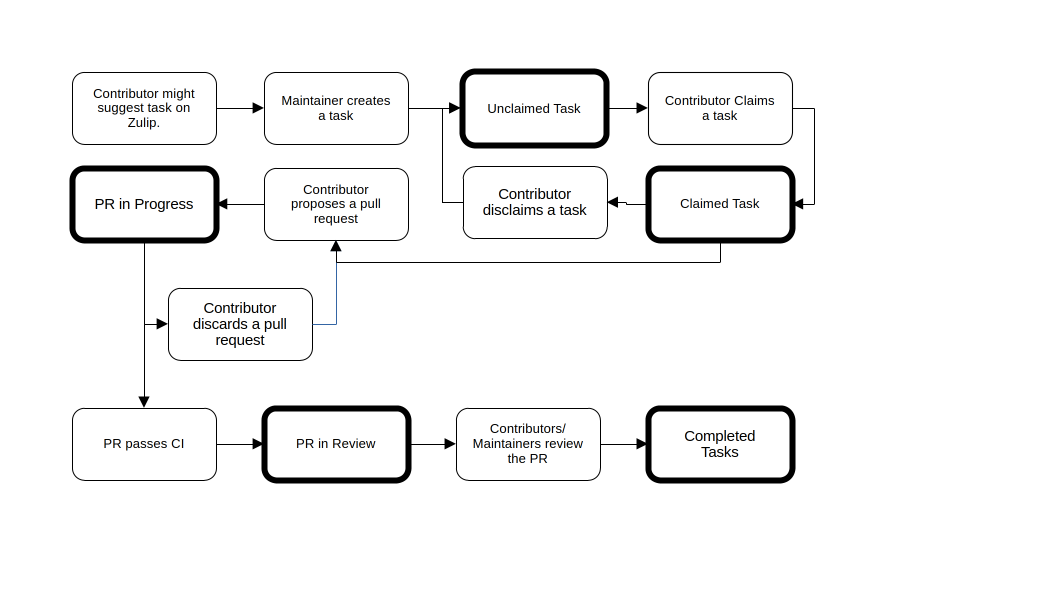
\includegraphics[width=1.0\textwidth]{proj_mgmt_figures/task_flowchart.png}
    \caption{\label{fig:proj_mgmt_flow} A partial flowchart of the automated task management process. Each task corresponds to an issue. A pull request is created to resolve tasks and once a pull request linked to a task is merged, the task is considered complete. The thick boxes represent states of the project dashboard represented by task columns. The movement of tasks between these states is automated by the CI which is triggered upon specific actions performed by contributors on the respective GitHub issues and pull requests. A more detailed description is found in the contributions file of the GitHub file, named CONTRIBUTING.md by convention.}
\end{figure}

\begin{figure}[t]
    \centering
    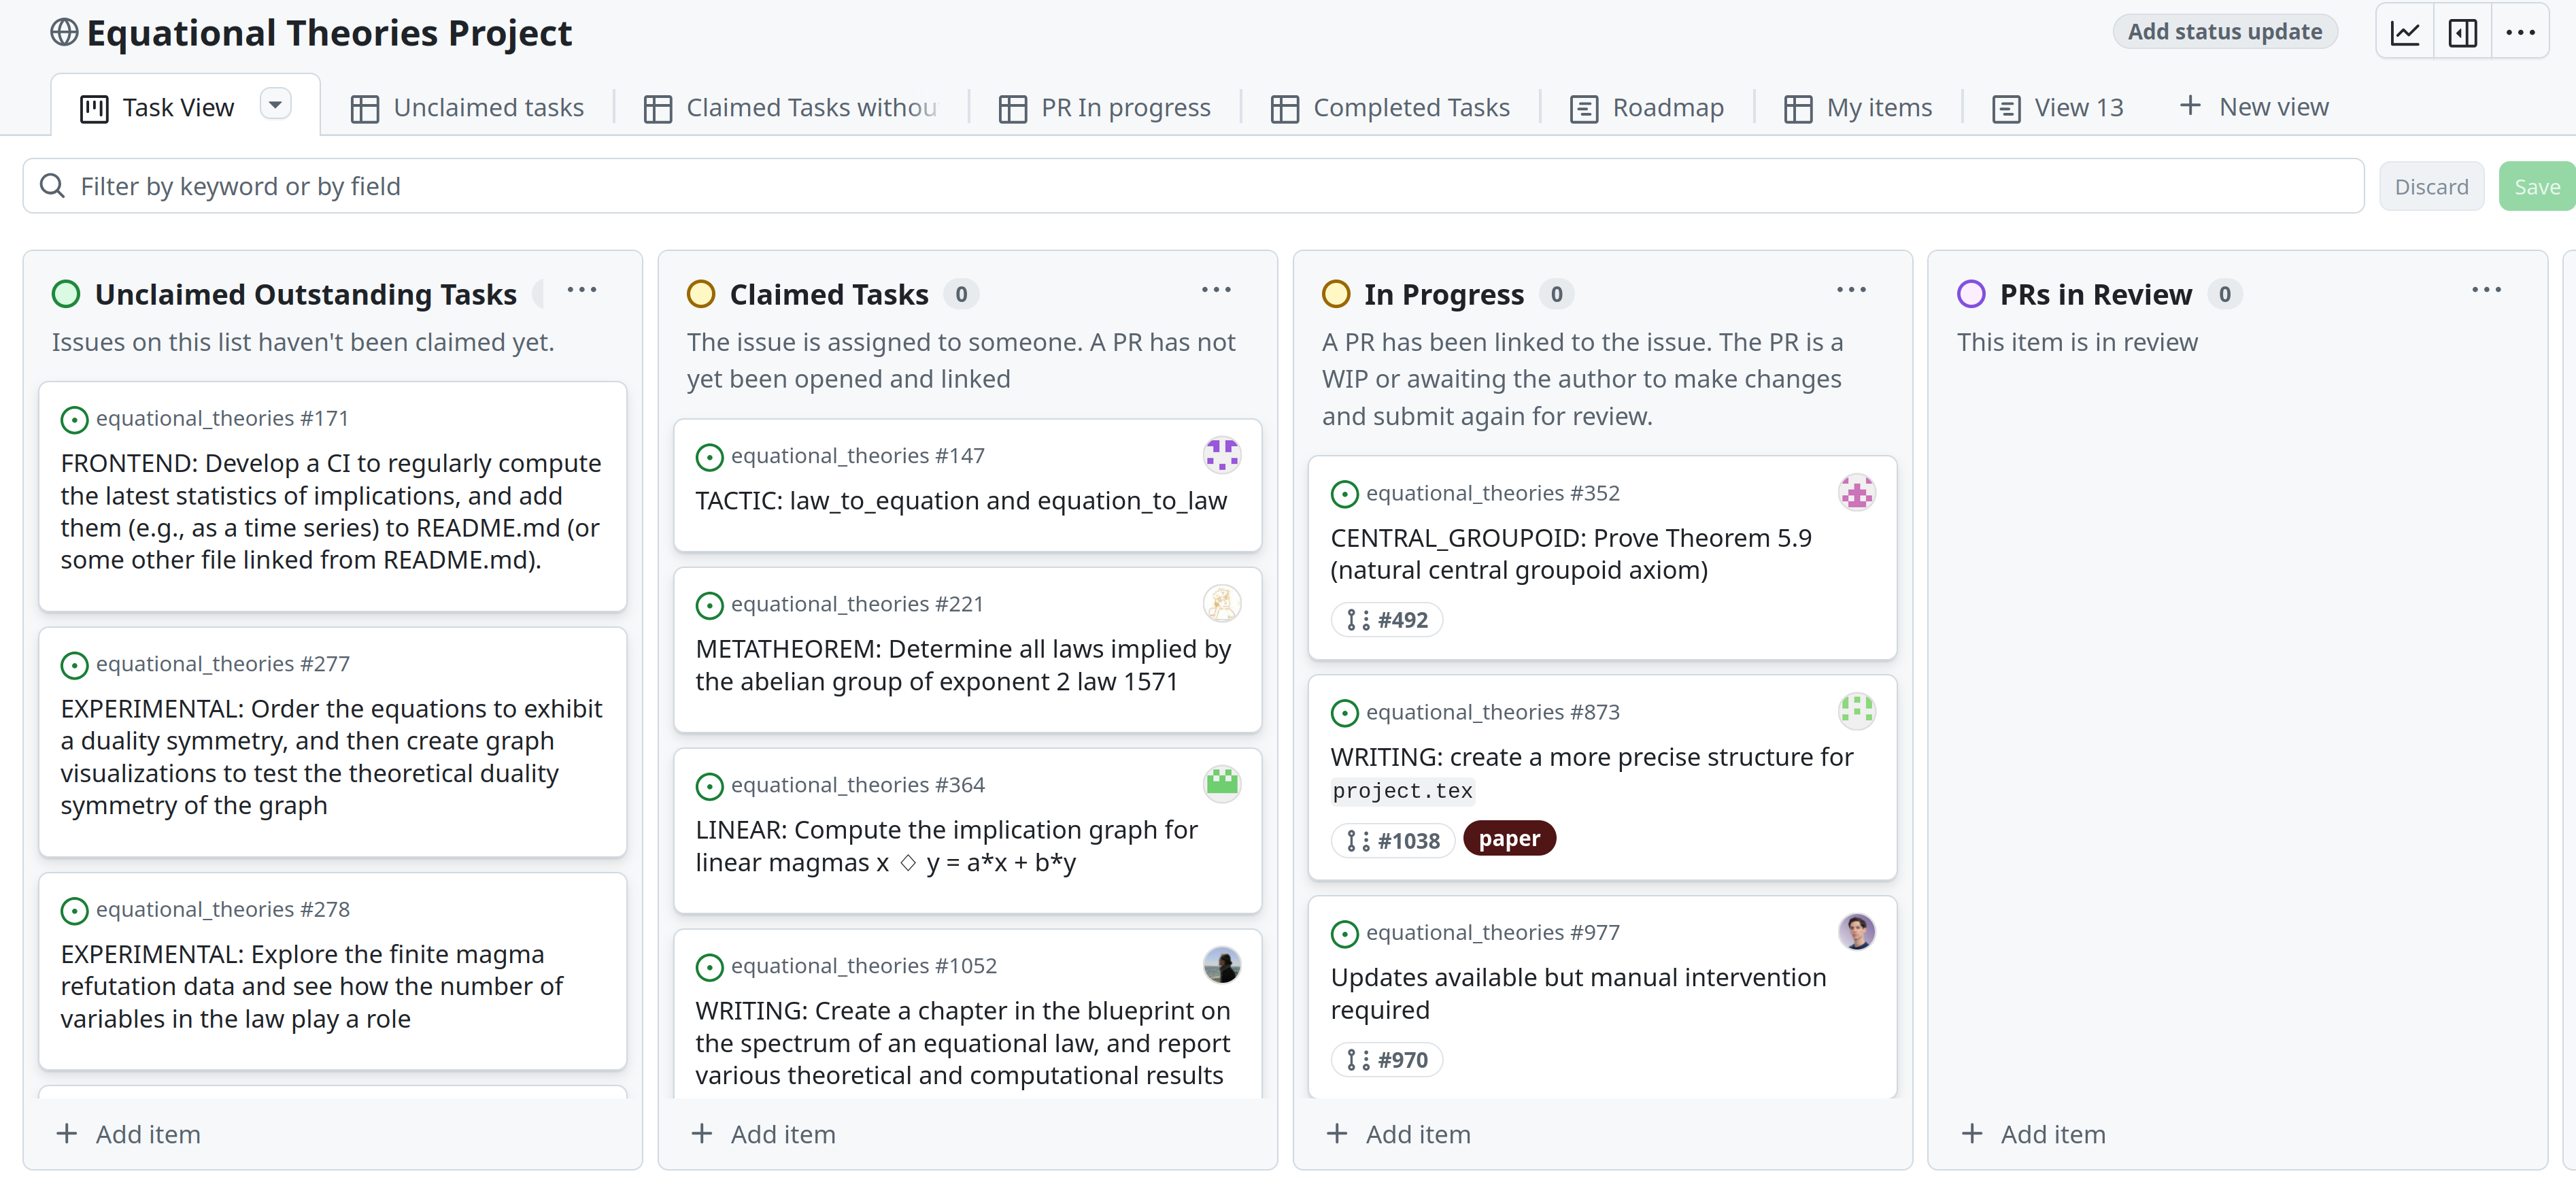
\includegraphics[width=1.0\textwidth]{proj_mgmt_figures/proj_dash_snapshot.png}
    \caption{\label{fig:proj_dashboard} A snapshot of the project dashboard as of July 30th 2025}
\end{figure}
\subsection{Trusting ITPs to Scale Collaboration}
In our project we used the interactive theorem prover (hereon ITP) lean 4 \cite{the_lean4_paper} precisely to address these issues of scaling. The contents of this section are common knowledge in the ITP and ITP-adjacent research communities. The exposition is intended to be useful to a user of ITPs.

At its core, an interactive theorem prover implements an expressive logic, encoded in a suitable choice of mathematical foundations. Lean 4 has the calculus of constructions extended by inductive types as its core logic. This logic is sufficiently powerful to express mathematical definitions and theorems for almost all areas of mathematical interest, while being relatively spartan and easy to write proof checkers for. Additionally, modern ITPs provide a convenient programming language which helps express mathematical ideas in a syntax closer to a mathematician's intuition than would be permitted by raw logical terms. A subset of ITPs like Lean, Rocq (formerly Coq), and Isabelle go one step further and provide the means to generate proofs through so-called \emph{tactics}. There are usually numerous tactics, each specialised for specific proof generation methods. Among other things, they search mathematical libraries, simplify expressions, and identify lemmas and hypotheses to make progress in proofs. The proofs generated by this overlying programming machinery are terms in the core logical calculus which are checked mechanically by the proof checker. But in a large project, there is more to trust. It helps to understand the nature and limits of trust one can place on ITPs.

For our purposes, lean consists of three pieces:
\begin{enumerate}
    \item A core proof checker called the \emph{kernel}. This checker encodes a typed $\lambda$-calculus that is sufficiently expressive for most mathematical purposes. Without getting into details, theorems are encoded as a formal specification of the intended theorem statement. Proofs are encoded as deduction trees using known lemmata, acceptable axioms, and inference rules. The kernel checks whether this deduction tree constitutes a correct deduction in the context of existing theorems and lemmata, called the \emph{environment}. Once a theorem's proof has been checked, it is added to the environment and can be used for constructing subsequent proofs. In reality, lean allows users some flexibility in adding declarations into its environment without checking their types.
    \item A sophisticated programming language in which users express their definitions and theorems. Programs in this language are said to  be \emph{elaborated} to produce definitions and proofs in the core logic that the kernel can check.
    \item A compiler which compiles executable lean code into reasonably efficient C code.
\end{enumerate}

Of these three pieces, \emph{the kernel is the smallest and most trusted piece}. Programs in the programming language are translated by an \emph{elaborator} to the spartan language of the kernel. In reality the elaborator does much more, but the key takeaways are the following:
\begin{itemize}
    \item The kernel only verifies programs of a very simple barebones language. A proof verified by Lean can be trusted \emph{modulo} the correctness of the kernel implementation. This caveat can be usually dropped because, the kernel is also one of the most battle-hardened pieces of an ITP.
    \item The kernel checks proofs against a given specification. This means that if the formal theorem statement itself is flawed or incorrectly uses other definitions, a correct and verified proof of this theorem would be mathematically meaningless. The formal statement of a theorem gives expression to a mathematician's intuition and intention, and as such, the only check against mistakes in this area come from human review. Lean cannot offer any guarantees against false statements written by its users or artificial intelligence tools.
    \item The higher level programming language can in-principle, generate arbitrary deductions. Their correctness is ultimately validated by the kernel. This gives the higher level programming language more leeway in generating possibly incorrect deductions.
    \item Ideally the environment only consists of definitions and lemmata already checked by the kernel. Thus their correct usage in the proof of subsequent theorems is valid. However this assumption is often not entirely true in practical implementations of theorem provers for efficiency reasons. In this case, trust in the kernel is restored by replaying each assumption from scratch in the kernel. This can be accomplished by external checkers. Such checkers, which are ideally independent implementations of the \emph{kernel}, can also guard against implementation mistakes in the kernel. In this project we used the environment replay tool \textit{lean4checker} and the \textit{lean4lean} \cite{lean4lean} tool. To our knowledge this was the first such use of the \textit{lean4lean} tool.

\end{itemize}

\begin{remark}
    A bug in the kernel that allows false statements to be proved is usually called a \emph{soundness} bug. Concretely, a soundness bug can be exploited to produce a kernel-certified proof of the proposition $False$. Such bugs are rare but not entirely non-existent. This is distinct from being able to proof $False$ by simply assuming contradictory or false statements. A proof of the proposition $False$ implies a proof of any statement by \emph{ex falso quod libet}.
\end{remark}

Users of lean only interact directly with the higher level programming language and usually get confirmation of the correctness of their proofs through the editor interface. Further, collaborators on a project such as ours are likely to deploy automated tools such as SAT solvers, SMT solvers, first-order theorem provers, and perhaps even modern AI tools. These tools usually produce proof certificates which are imported or inserted into a lean source files. Some modern AI tools are integrated into code editors which might automatically produce or edit even the statements of theorems and the definitions they deal with. Given the limits to trust mentioned above, a productive and useful collaboration using lean also requires a collaboration and verification infrastructure combining human effort and automated tools. It is in this context that we discuss the project infrastructure. It is a concrete answer to the questions posed by one of the authors at the beginning of this project \cite{Tao_blog_Sep_2024} that combines tools from the ITP community and the software engineering community. All these tools already exist. The goal of this exposition is to explain how they address the concerns described above.


\paragraph{\textbf{The non-lean pieces:}} While lean can check proofs of theorems upto the limitations described above, a project of this scale involves the use of several non-lean tools. For example there are tools which extract the proven implications and anti-implications. There are tools which construct various visualisations. There are also metaprograms which call external automated theorem provers, and extract proof certificates from them to construct a lean proof out of them. In keeping with the garbage-in garbage-out principle, if these tools get spurious inputs and throw spurious outputs, lean can only tell us that the proofs are incorrect after the formal proofs have been translated to lean. It cannot, for instance, stop us from generating a large number of spurious conjectures that misguide contributors because of a simple index error in an array. Further, the continous integration scripts that run lean and check the lean code with external checkers are not formally verified. Such bugs can only be unconvered by empirical testing and user reports. This highlights a basic caveat when using interactive theorem provers. These tools checks something highly specific, a proof, against a specification. Contributors are responsible for the correctness of everything else. This makes the role of organisers and maintainers especially important.

\subsection{The Role of Organisers and Maintainers}
As mentioned before, the correctness of the project depends on a lot of moving pieces, many of which cannot be guaranteed to be correct or functional by lean. In this section, we give a brief description of the variety of tasks that need to be performed by maintainers. We wish to emphasise that the role played by maintainers is akin to that played by the principal investigator and senior postdoctoral researchers in a large experimental project, in that they need to understand the big picture and mathematical details of the project to a reasonable extent and be capable of making highly technical decisions, either themselves, on in consultation with subject experts. Further, they are likely to have limited time to get involved in highly specific details of the project, and while they might make technical contributions, most of their time will be spent managing and organising tasks for other contributors. The role requires a  combination of mathematical research skills and capacity with software engineering tools.

The organisers and maintainers have several tasks in a project such as ours.
\begin{itemize}
    \item They are responsible for monitoring the Zulip chat and onboarding new contributors.
    \item They are responsible for creating new tasks based on requirements and Zulip discussions, and ensuring that they are properly assigned.
    \item They are responsible for ensuring that all the project automation functions smoothly and step in when an issue is detected. It greatly helps to have a geographically distributed set of maintainers across timezones to help fix issues at any time of the day.
    \item They are responsible for the early design decisions, such as good definitions or top-level theorem statements in the project that are most likely to incur technical debt. For instance, we started with a definition of free magmas that competed with the one in Mathlib. This needless redundancy meant that we could not freely import all of Mathlib, a normal practice during the coding process in lean projects. Given the extremely fast progress in the initial days of the project, it became hard to review and later alter this design decision.
    \item They are responsible for reviewing all code, both lean proofs and theorems, and non-lean scripts. This includes ensuring that the automation to build and check proofs, compile the documentation and blueprint, and test and run scripts works smoothly. When necessary they must be willing to step in and build or repair the automation.
    \item They are responsible for reviewing and developing the basic definitions and theorems. As mentioned before, lean takes definitions and theorems for granted. Thus maintainers need to be familiar with both the mathematical content and good ways of expressing this content in lean. Being proficient in lean internals is helpful for maintainers in identifying anti-patterns like the use of certain tactics that lead to trusting the lean compiler, such as \texttt{native\_decide}.
    \item Maintainers are responsible for helping contributors who might get stuck in a proof. Other contributors may also assist in such matters, but ultimately it is up to the maintainers to ensure progress.
    \item Experienced maintainers might also offer suggestions and guidance on how to produce shorter or more elegant proofs.
    \item They are responsible for ensuring that some basic standards are met in proof blocks that make proofs robust to upstream changes. For instance, non-terminal uses of the \texttt{simp} tactic must be replaced with the \texttt{simp only} tactic with an explicit list of lemmas used. Otherwise, changes in the behaviour of upstream libraries can change how the tactic works and affect the correctness of the proof, when the lean toolchain is updated.
    \item They are responsible for maintaining some record of the progress of the project, Projects on this scale can take a long time and it can become hard to remember how the project progressed. It would be extremely tedious to try to reconstruct real-time impressions long after the fact just from the GitHub commit history and Zulip chat archive. Thus it is extremely helpful if maintainers keep and publish regular logs of activities at a frequency that is proportionate to the scale of activity in the project.In our case, the main organiser maintained a daily log of activities during the busiest part of the project, which became less frequent as the project progress rate slowed towards the end.
\end{itemize}

In this project, we were still learning a lot of the aforementioned lessons. A key learning from this project is that it really helps to have a maintainer structure in place before the project begins, rather than inventing one on the fly. Of course, new contributors can be onboarded as maintainers as necessary. But a small maintainer team in the initial stages can hamper proper review processes and result in suboptimal design choices in the lean formalization that become hard to undo later, as was the case with the aformentioned free magma issue. As another example, the initial list of equations were translated and put into one lean file as opposed to several. This created excessively large lean files which could have been managed better with a better file organisation.

In conclusion, we wish to emphasise that at projects scale, the administrative aspects of the project assume non-trivial importance. They require people who are proficient in at least part of the research topic, technical tools, and administrative matters. Setting these processes well in advance of announcing the project and inviting contributors leads to a smoother project.





\begin{comment}
-- The below should be in the metatheory section.

Use of transitive reduction etc.\ to keep the Lean codebase manageable. Note that the project is large enough that one cannot simply accept arbitrary amounts of Lean code into the codebase, as this could make compilation times explode. Also note somewhere that transitive completion can be viewed as directed graph completion on a doubled graph consisting of laws and their formal negations.
\end{comment}
